\documentclass[a4paper,11pt]{book}

\usepackage[T1]{fontenc}
\usepackage[utf8]{inputenc}
\usepackage[LGR,T1]{fontenc} % notice LGRx instead of LGR
\usepackage{lmodern}
\usepackage[final]{pdfpages} 
\usepackage[top=2cm, bottom=3cm, outer=3cm, inner=4cm, headsep=14pt]{geometry}
\usepackage{textgreek}
\usepackage{csquotes}
\usepackage[french]{babel}
\usepackage{fancyhdr}
\usepackage{xsim}
\usepackage{tasks}
\usepackage[absolute]{textpos}
\usepackage{ascii}
\usepackage{eurosym}
\usepackage{amsthm}

\theoremstyle{definition}
\newtheorem{exmp}{Example}[section]

\bibliographystyle{abbrv}
\pagestyle{fancy}
\fancyhf{}
\renewcommand{\footrulewidth}{1pt}
\renewcommand{\thesection}{\arabic{section}}

\lhead{Architecture des ordinateurs}
\rhead{Représentation binaire}
\rfoot{Page \thepage}

\begin{document}

\chapter{Représentation binaire}
\section{Introduction}
La représentation binaire de l'information va nous permettre une représentation physique de l'information traduite dans deux états distincts. Dans les systèmes informatiques, il s'agit presque toujours d'une représentation avec deux tensions distinctes, mais on pourrait imaginer l'utilisation d'autres états physiques. C'est par exemple le cas dans le stockage sur des supports magnétiques où l'on utilise des orientations distinctes du champ. Des réalisations mécaniques, peu commodes ou irréalistes ont aussi été proposées comme un système avec des cordes et des poulies dans \cite{ordiantique}.

Le choix binaire est également une commodité choisie arbitrairement. Ainsi les Russes avaient conçu en 1958 un ordinateur : l'ordinateur Setun qui travaillait en base trois. Depuis le début du 21e siècle, on développe également des ordinateurs quantiques basés sur des états quantiques superposés.

Il existe différentes façon de représenter de l'information. On parle de représentation pour des nombres, des images. On parle de format pour définir la structuration de l'information et d'encodage pour la représentation "atomique" des éléments de l'information. Dans ce chapitre, nous allons surtout nous intéresser aux différents encodages possibles.

\subsection{Bases : notions générales}
Quelle que soit la base, un nombre est représenté par une suite de chiffres. Ainsi en base dix, 10 vaut 10, alors qu'en base deux, 10 (que l'on prononcera un-zéro) vaut 2, en base quatre, 10 (un-zéro) vaut 4, etc. Plus loin, en base dix, 100 vaut 100, alors qu'en base deux 100 (un-zéro-zéro) vaut 4.

À partir de là, nous pouvons poser une expression généralisée d'un nombre dans une base $B$ quelconque, nous avons tout d'abord les chiffres utilisés qui vont de 

\[0 \rightarrow B-1\].
\\
\textit{Exemple : } 0, 1, 2, 3 en base 4.\\

L'expression d'un nombre par une suite de chiffres :

\[C_n C_{n-1} ... C_1 C_0\]

nous donne un nombre : 

\[C_n \times B^n + C_{n-1} \times B^{n-1} + ... + C_1 \times B^1 + C_0 \times C^0\]

\subsubsection{Exemple}

Prenons le nombre composé de quatre chiffres : 1101. Exprimé en base B, ce nombre s'analyse :

\[ 1\times B^{3}+1\times B^{2}+0\times B^{1}+1\times B^{0} \]

Ce qui donne :
\begin{itemize}
    \item 1101 en base $B = 10$ : $1\times 10^{3}+1\times 10^{2}+0\times 10^{1}+1\times 10^{0} = 1101 $
    \item 1101 en base $B = 8$ : $1\times 8^{3}+1\times 8^{2}+0\times 8^{1}+1\times 8^{0} = 577$
    \item 1101 en base $B = 2$ : $1\times 2^{3}+1\times 2^{2}+0\times 2^{1}+1\times 2^{0} = 13$
\end{itemize}

\subsubsection{Bases supérieures à dix}
Das le cas des Bases supérieures à dix, nous rencontrons le problème du nombre de chiffres disponibles. C'est notamment le cas de l'hexadécimal (base seize) très utilisé en informatique. Dans ce cas nous ajoutons des chiffres représentés par les premières lettres de l'alphabet.
Ainsi en hexadécimal, nous avons l'ensemble des chiffres C:

\[C = \{0,1,2,3,4,5,6,7,8,9,A,B,C,D,E,F\}\]

\subsubsection{Exemples}
\begin{itemize}
    \item \[A0 \rightarrow 160\]
    \item \[FF \rightarrow 255\]
\end{itemize}

Le système hexadécimal est largement utilisé en informatique car il permet une notation compacte et une conversion sans calcul. En effet, 16 est une puissance de 2 ($2^4$), un chiffre en base 16 correspond donc à un nombre de 4 chiffres en base 2. Un octet (séquence de huit chiffres\footnote{On parle de huit bit, bit étant l'abréviation en anglais de BInary digiT. Un octet est donc composée de huit bits}) en base 2 peut donc toujours s'exprimer avec 2 chiffres en hexadécimal.

\subsubsection{Notations hexadécimales}
Il existe plusieurs façons d'indiquer qu'un nombre est exprimé en hexadécimal
\begin{itemize}
    \item Notations préfixées
    \begin{itemize}
        \item 0xA0 (language C)
        \item \&h123 (BASIC)
        \item \$123 (en Pascal)
        \item 0h123 (Texas Instrument)
        \item X'123' (COBOL)
    \end{itemize}
    \item Notations suffixées (utilisées en arithmétique)
    \begin{itemize}
        \item 123h
        \item $123_{(16)}$
    \end{itemize}
\end{itemize}

\begin{exercise}
    Convertir en base dix les nombres suivants.
    \begin{tasks}(3)
        \task $10_{(8)}$
        \task $10_{(16)}$
        \task $FF_{(16)}$
    \end{tasks}
\end{exercise}

\subsection{Code Décimal, Codé Binaire (BCD)}
Le code décimal, codé binaire (BCD)\footnote{Binary Coded Decimal} est l'encodage le plus répandu avec le complément à deux que nous verrons plus loin. C'est une traduction directe d'un nombre de la base dix à la base deux. On décompose ainsi le nombre décimal en puissance de deux. On parle de code 8421 car les 4 bits pondèrent les nombres 8, 4, 2 et 1 respectivement. Il existe d'autres façons d'organiser les bits\footnote{En particulier la notation 2421 qui permet d'encoder des nombres de 0 à 9, codage utile pour la représentation sur des dispositifs 7 segments que nous verrons au dernier chapitre.}, mais de manière générale, sur un octet, on garde un ordre du plus grand au plus petit de gauche à droite, les autres organisations restant des cas très spécifiques. Par contre, une fois les bits regroupés par octets, il existe de nombreuses façon de représenter les plus grands nombres, on parlera par exemple d'architecture LITTLE ENDIAN ou BIG ENDIAN, nous verrons cela plus loin.
On obtient ainsi la table \ref{table:codeBCD}.
\begin{table}[h!]
\centering
\begin{tabular}{ |c|c| } 
 \hline
 Chiffre & Bits  \\ 
 \hline
 0 & 0000  \\ 
 1 & 0001  \\ 
 2 & 0010  \\ 
 3 & 0011  \\ 
 4 & 0100  \\ 
 5 & 0101  \\ 
 6 & 0110  \\ 
 7 & 0111  \\ 
 8 & 1000  \\ 
 9 & 1001  \\ 
 10 & 1010  \\ 
 11 & 1011  \\ 
 12 & 1100  \\ 
 13 & 1101  \\ 
 14 & 1110  \\ 
 15 & 1111  \\ 
 \hline
\end{tabular}
\caption{Encodage BCD 8421}
\label{table:codeBCD}
\end{table}


Cela permet d’écrire la séquence 123 : 0001 0010 0011. Attention, le nombre 123 lui s'écrira : \[0111 1011\] ce qui se vérifie facilement : \[2^6 + 2^5 + 2^4 + 2^3 + 2^1 + 2^0 = 64 + 32 + 16 + 8 + 2 + 1 = 123 \]

\textbf{Multiplication par deux :} Pour multiplier par deux en binaire, il faut simplement décaler le nombre à gauche. C'est exactement similaire à la multiplication par dix en base dix. Par exemple: $0110_{binaire} (4 + 2 = 6_{decimal})$ devient $1100_{binaire} (8 + 4 = 12_{decimal})$.

\textbf{Division (entière) par deux (sans reste):} Pour diviser par deux en binaire, il faut simplement décaler le nombre à droite (inverse de la multiplication) en laissant disparaître les bits qui "sortent". Comme exemple, on peut simplement diviser douze par deux et vérifier que l'exemple ci-dessus fonctionne. Pour un nombre impair : $0101_{binaire} (4 + 1 = 5_{decimal})$ devient $0010_{binaire} (2_{decimal})$.
\\
\\
Le grand intérêt du système BCD pour l’électronicien est la possibilité de
manipuler les chiffres en base dix pour différentes fins, notamment l’affichage, comme ce sera illustré dans les chapitres suivants.

\begin{exercise}
    Convertir les nombres décimaux suivants en binaire.
    \begin{tasks}(3)
        \task 3
        \task 5
        \task 8
        \task 19
        \task 126
        \task 146
    \end{tasks}
\end{exercise}

\begin{exercise}
    Convertir les nombres binaires suivants en décimal.
    \begin{tasks}(3)
        \task 0011
        \task 0101
        \task 1000
        \task 0001 0011
        \task 1000 0000
        \task 1001 0010
    \end{tasks}
\end{exercise}


\subsection{Codage de Gray}
Comme nous aurons le temps de l’apprécier plus tard, un des problèmes importants des systèmes numériques tient dans la synchronisation des différents signaux numériques. Lorsque l’on conçoit un compteur, ce problème devient important car dans la représentation binaire des nombres entiers, il arrive souvent que plusieurs bits changent en même temps. Or pour différentes raisons, plus communément des questions de \textit{temps de propagation}, les transitions peuvent se "décaler". Dans ce cas, il est possible que des nombres non désirés apparaissent dans le compte (l'exercice \ref{propagation} illustre parfaitement ce problème).
Considérons l’exemple suivant. Nous voulons concevoir un compteur trois bits, en faisant varier trois signaux, v0, v1, v2 :
\begin{figure}[h]
\centering
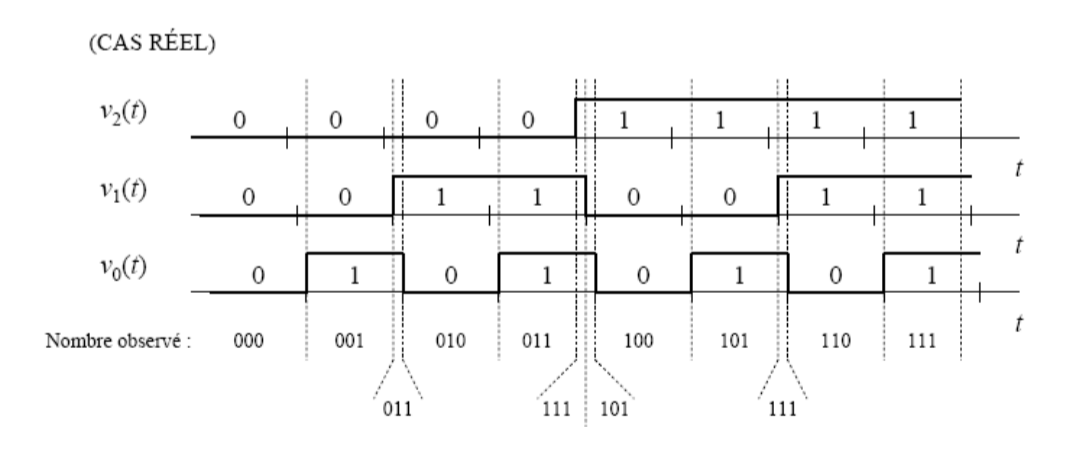
\includegraphics[width=0.5\textwidth]{media/SignauxBinaires_Sync.png}
\caption{Signaux binaires}
\end{figure}

Notons au passage qu'un système synchrone ne souffrira pas de ce genre de problème. C'est pour cela que dans un microprocesseur on utilise facilement le codage BCD puisque la synchronicité est assurée par un signal d'horloge (CLK).

Ce problème survient également dans les systèmes de comptage opto-mécanique utilisés pour déterminer des angles rotation dans une machine. Si le dispositif se salit (poussière, éclaboussure), on ne peut pas facilement détecter l'erreur.

Le codage de Gray propose une solution ou un seul bit change à chaque incrément. De cette façon, on adresse les deux problèmes évoqués : pas besoin de synchroniser les changements de bits, un changement de deux bits révèle immédiatement une erreur de lecture.

Ce code a été inventé par Frank Gray au \textit{Bell Lavs} et breveté en 1953.

\begin{table}[h!]
\centering
\begin{tabular}{ |c|c|c| } 
 \hline
 Décimal & Binaire & Gray  \\ 
 \hline
 0 & 0000 & 0000  \\ 
 1 & 0001 & 0001 \\ 
 2 & 0010 & 0011 \\ 
 3 & 0011 & 0010 \\ 
 4 & 0100 & 0110 \\ 
 5 & 0101 & 0111 \\ 
 6 & 0110 & 0101 \\ 
 7 & 0111 & 0100 \\ 
 8 & 1000 & 1100 \\ 
 9 & 1001 & 1101 \\ 
 10 & 1010 & 1111 \\ 
 11 & 1011 & 1110 \\ 
 12 & 1100 & 1010 \\ 
 13 & 1101 & 1011 \\ 
 14 & 1110 & 1001 \\ 
 15 & 1111 & 1000 \\ 
 \hline
\end{tabular}
\caption{Codage de Gray}
\label{table:1}
\end{table}

On remarquera de plus que l'on peut recommencer le comptage de manière circulaire en respectant la règle du un seul bit qui change: 

\[15 \rightarrow 0 \Leftrightarrow 0100 \rightarrow 0000\]

Ce qui nous permet d'encoder des disques pour la mesure de rotation angulaire dans une machine. On notera également les symétries qui apparaissent dans le codage de Gray sur la figure \ref{codeGray}. Ce détail peut servir d'aide pour retrouver la table d'encodage, et on appelle également le codage de Gray \textit{code binaire réfléchi}. Ainsi, pour "construire" un codage de Gray, on commence simplement avec 0 et 1, puis chaque fois que c'est nécessaire, on ajoute un bit à gauche en reprenant l'énumération des nombres précédents dans le sens inverse, on construit ainsi une table symétrique avec un 1 comme bit situé le plus à gauche.


\begin{figure}[h]
\centering
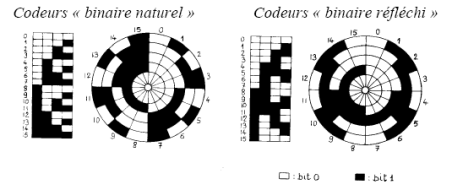
\includegraphics[width=0.5\textwidth]{media/comparaison_codes_binaires.png}
\caption{Capteurs binaires}
\label{codeGray}
\end{figure}


Nous utiliserons cette propriété de ne changer qu'un seul bit dans un espace circulaire plus loin, en particulier dans les tables de Karnaugh.

\begin{exercise} Temps de propagation
    \begin{tasks}(1)
        \task Soit un signal d'horloge à 3GHz, quelle est la durée d'une période du signal ?
        \task Soit deux lignes différentes d'un même bus (servant par exemple à interconnecter le processeur et la RAM), une des lignes mesures 4cm et l'autre 2cm. Pour simplifier, prenons un temps de propagation égal à $c$ (vitesse de la lumière). Calculez le temps de propagation du signal sur ces deux lignes et mettez en évidence la différence en rapport avec la période du signal calculée précédemment.

    \end{tasks}
    \label{propagation}
\end{exercise}

        \begin{figure}[h]
            \centering
            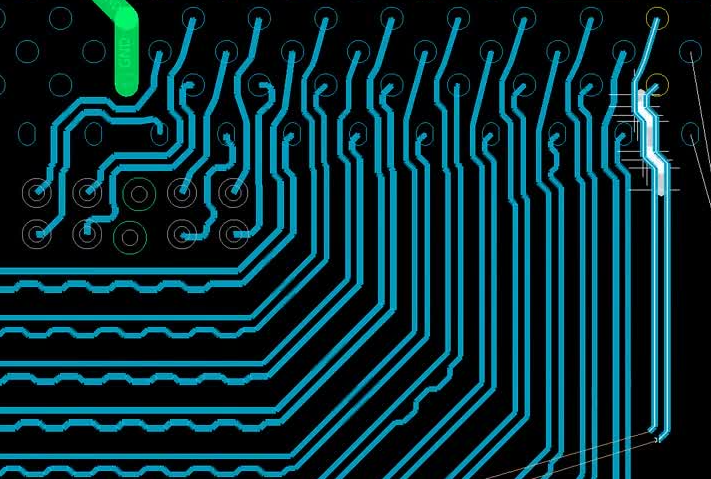
\includegraphics[width=0.5\textwidth]{media/buslines.png}
            \caption{Lignes de circuit sur un plan de PCB}
            \label{codeGray}
        \end{figure}


\subsubsection{Transcodage binaire $\rightarrow$ Gray}
La formule pour obtenir le code de Gray à partir du binaire pur est la suivante (méthode de l'addition décalée sans retenue):

\[N_{Gray} = \frac{N_{binaire}\oplus2N_{binaire}}{2}\]
\\
\textbf{Exemple complet :} soit $N_{binaire} = 0111$, on a $2N = 1110$, $N\oplus2N = 0111 \oplus 1110 = 1001$, que l'on divise par deux : $\frac{1001}{2}= 0100$ le code de Gray de sept en décimal.

\begin{exercise}
    Trouver le codage de Gray pour les nombres décimaux suivants :
    \begin{tasks}(3)
        \task 7
        \task 9
        \task 15
        \task 2
        \task 5
        \task 11
    \end{tasks}
\end{exercise}

\subsubsection{Transcodage Gray $\rightarrow$ binaire}
Pour la conversion de Gray vers binaire, on va cette fois lire le nombre de droite à gauche (du bit le plus significatif \textit{Most Significant Bit, MSB} vers le bit le moins significatif \textit{Less Significant Bit, LSB}).
Le premier bit (le plus à gauche) est strictement identique. Ensuite, si le bit suivant dans le code de Gray est à zéro, on recopie le bit précédent, s'il est à un, on l'inverse.

\textbf{Exemple 1 :} Nous avons $0100_{Gray}$. 

$0 \rightarrow 0$

$1 \rightarrow 1$ (on change le bit précédent puisque nous avons un 1).

$0 \rightarrow 1$ (on recopie le bit précédent)

$0 \rightarrow 1$

Soit : $0111_{BCD}$ ce qui fait 7 en décimal.

\textbf{Exemple 2 :} Nous avons $01101_{Gray}$. 

$0 \rightarrow 0$

$1 \rightarrow 1$ (on change le bit précédent puisque nous avons un 1).

$1 \rightarrow 0$ (on change le bit précédent puisque nous avons un 1).

$0 \rightarrow 0$ (on recopie le bit précédent).

$1 \rightarrow 1$ (on change le bit précédent puisque nous avons un 1).

Soit : $ 01001_{BCD}$ ce qui fait 9 en décimal.

\begin{exercise}
    À partir des nombres en codage de Gray suivants, trouver la représentation BCD et le nombre décimal correspondants :
    \begin{tasks}(3)
        \task 0100
        \task 1111
        \task 0101
        \task 0011
        \task 1000
        \task 1001
    \end{tasks}
\end{exercise}

\subsection{Code avec complément à deux}
De manière générale, on définit la soustraction comme une addition du négatif du deuxième opérante:
\[A -B \Leftrightarrow A + (-B)\]
Pour pouvoir introduire la soustraction, il nous faut donc commencer par proposer une représentation des nombres négatifs.

\subsubsection{Le bit de signe}
Une première solution, simpliste, serait d'utiliser le bit de poids le plus fort (çàd. le bit le plus à gauche) comme bit de signe.
\\
Ainsi, pour -3 nous aurions: 1000 0011.\\
Cette solution pose cependant problème:
\\
\\
\begin{tabular}{ c|c }
 3 & 0000 0011 \\
 -3 & 1000 0011 \\
 \hline
 ?? & ?? \\
\end{tabular}
\\
\\
La soustraction ne se transforme pas en une addition simple.

\subsubsection{Le complément à 1}
Le complément à 1 s'obtient simplement en inversant tous les bits. Nous verrons plus loin qu'il est de plus facile de mettre en place un circuit logique pour effectuer cette opération. Nous obtenons alors:
\\
\\
\begin{tabular}{ c|c }
 3 & 0000 0011 \\
 -3 & 1111 1100 \\
 \hline
 -0 & 1111 1111 \\
\end{tabular}
\\
\\
Cette solution fonctionne, mais elle présente un désavantage, nous avons en effet deux représentations pour o (littéralement 0 et -0) : 0000 0000 et 1111 1111.
On voit cependant qu'il suffirait d'ajouter 1 à -0 pour retomber sur +0 en ignorant le retenue en dépassement.

\subsubsection{Le complément à 2}
Le complément à deux s'obtient donc en inversant tous les bits et en ajoutant 1 pour obtenir un nombre négatif. Nous obtenons ainsi :
\\
\\
\begin{tabular}{ c|c }
 3 & 0000 0011 \\
 -3 & 1111 1101 \\
 \hline
 -0 & 0000 0000 \\
\end{tabular}
\\
\\
Ce qui est la meilleure solution que nous allons donc retenir pour la représentation des nombres négatifs.

Cette opération correspond au calcul de \[ 2^n - |x| \] où n est la longueur de la représentation et \[ |x| \] la valeur absolue du nombre à coder. 
Ainsi, -1 s'écrit comme 256 - 1 = 255 = $1111 1111_{2}$, pour les nombres sur 8 bits. Ceci est à l'origine du nom de cette opération : "complément à 2 puissance n", quasi-systématiquement tronqué en "complément à 2".

On notera encore que l'opération est réversible. 

Ainsi :
$-3 \rightarrow 1101; -(-3) \rightarrow 0011 \rightarrow 3$


Avec un mot de n bits, il est possible de représenter les valeurs de $-2n-1$ à $2n-1-1$ et il n'existe qu'une représentations possible pour la valeur 0.

\begin{exercise}
    Calculer la valeur min et la valeur max que l'on peut coder avec des mots de 8 bits (un octet).
\end{exercise}

\begin{exercise}
    Convertir les nombres décimaux suivants en binaire, complément à deux.
    \begin{tasks}(3)
        \task -3
        \task -5
        \task -8
        \task -19
        \task -126
        \task -127
    \end{tasks}
\end{exercise}

\begin{exercise}
    Effectuer en binaire les opérations suivantes.
    \begin{tasks}(3)
        \task 5 - 3
        \task 3 - 5
        \task 8 - 8
        \task 32 - 19
        \task 12 - 4
        \task 0 - 126
    \end{tasks}
\end{exercise}

\subsection{Code ASCII}
Le Code ASCII (acronyme de Américan Standard Code for Information Interchange) est l’un des plus anciens et certainement le plus largement utilisé des codes représentatifs. Le tableau suivant énumère quelques caractères du code ASCII

  \begin{tabular}{ |cccc| }
    \hline
    000\textit{d} & 00\textit{h} & \NUL & (nul) \\
    001\textit{d} & 01\textit{h} & \SOH & (soh) \\
    002\textit{d} & 02\textit{h} & \STX & (stx) \\
    003\textit{d} & 03\textit{h} & \ETX & (etx) \\
    004\textit{d} & 04\textit{h} & \EOT & (eot) \\
    005\textit{d} & 05\textit{h} & \ENQ & (enq) \\
    006\textit{d} & 06\textit{h} & \ACK & (ack) \\
    007\textit{d} & 07\textit{h} & \BEL & (bel) \\
    008\textit{d} & 08\textit{h} & \BS  & (bs)  \\
    009\textit{d} & 09\textit{h} & ~    & (tab) \\
    010\textit{d} & 0A\textit{h} & \LF  & (lf)  \\
    011\textit{d} & 0B\textit{h} & \VT  & (vt)  \\
    012\textit{d} & 0C\textit{h} &  ~   & (np)  \\
    013\textit{d} & 0D\textit{h} & \CR  & (cr)  \\
    014\textit{d} & 0E\textit{h} & \SO  & (so)  \\
    015\textit{d} & 0F\textit{h} & \SI  & (si)  \\
    \hline
  \end{tabular}
    \begin{tabular}{ |cccc| }
    \hline
    016\textit{d} & 10\textit{h} & \DLE & (dle) \\
    017\textit{d} & 11\textit{h} & \DCa & (dc1) \\
    018\textit{d} & 12\textit{h} & \DCb & (dc2) \\
    019\textit{d} & 13\textit{h} & \DCc & (dc3) \\
    020\textit{d} & 14\textit{h} & \DCd & (dc4) \\
    021\textit{d} & 15\textit{h} & \NAK & (nak) \\
    022\textit{d} & 16\textit{h} & \SYN & (syn) \\
    023\textit{d} & 17\textit{h} & \ETB & (etb) \\
    024\textit{d} & 18\textit{h} & \CAN & (can) \\
    025\textit{d} & 19\textit{h} & \EM  & (em)  \\
    026\textit{d} & 1A\textit{h} & ~    & (eof) \\
    027\textit{d} & 1B\textit{h} & \ESC & (esc) \\
    028\textit{d} & 1C\textit{h} & \FS  & (fs)  \\
    029\textit{d} & 1D\textit{h} & \GS  & (gs)  \\
    030\textit{d} & 1E\textit{h} & \RS & (rs)  \\
    031\textit{d} & 1F\textit{h} & \US & (us)  \\
    \hline
  \end{tabular}
  \begin{tabular}{|ccc|}
    \hline
    032\textit{d} & 20\textit{h} & \textvisiblespace  \\
    033\textit{d} & 21\textit{h} & ! \\
    034\textit{d} & 22\textit{h} & " \\
    035\textit{d} & 23\textit{h} & \# \\
    036\textit{d} & 24\textit{h} & \$ \\
    037\textit{d} & 25\textit{h} & \% \\
    038\textit{d} & 26\textit{h} & \& \\
    039\textit{d} & 27\textit{h} & \textquotesingle \\
    040\textit{d} & 28\textit{h} & ( \\
    041\textit{d} & 29\textit{h} & ) \\
    042\textit{d} & 2A\textit{h} & * \\
    043\textit{d} & 2B\textit{h} & + \\
    044\textit{d} & 2C\textit{h} & \textquoteright \\
    045\textit{d} & 2D\textit{h} & - \\
    046\textit{d} & 2E\textit{h} & . \\
    047\textit{d} & 2F\textit{h} & / \\
    \hline
  \end{tabular}
  \begin{tabular}{|ccc|}
    \hline
    048\textit{d} & 30\textit{h} & 0 \\
    049\textit{d} & 31\textit{h} & 1 \\
    050\textit{d} & 32\textit{h} & 2 \\
    051\textit{d} & 33\textit{h} & 3 \\
    052\textit{d} & 34\textit{h} & 4 \\
    053\textit{d} & 35\textit{h} & 5 \\
    054\textit{d} & 36\textit{h} & 6 \\
    055\textit{d} & 37\textit{h} & 7 \\
    056\textit{d} & 38\textit{h} & 8 \\
    057\textit{d} & 39\textit{h} & 9 \\
    058\textit{d} & 3A\textit{h} & : \\
    059\textit{d} & 3B\textit{h} & ; \\
    060\textit{d} & 3C\textit{h} & < \\
    061\textit{d} & 3D\textit{h} & = \\
    062\textit{d} & 3E\textit{h} & > \\
    063\textit{d} & 3F\textit{h} & ? \\
    \hline
  \end{tabular}
\\
\\
  
  \begin{tabular}{|ccc|}
    \hline
    064\textit{d} & 40\textit{h} & @ \\
    065\textit{d} & 41\textit{h} & A \\
    066\textit{d} & 42\textit{h} & B \\
    067\textit{d} & 43\textit{h} & C \\
    068\textit{d} & 44\textit{h} & D \\
    069\textit{d} & 45\textit{h} & E \\
    070\textit{d} & 46\textit{h} & F \\
    071\textit{d} & 47\textit{h} & G \\
    072\textit{d} & 48\textit{h} & H \\
    073\textit{d} & 49\textit{h} & I \\
    074\textit{d} & 4A\textit{h} & J \\
    075\textit{d} & 4B\textit{h} & K \\
    076\textit{d} & 4C\textit{h} & L \\
    077\textit{d} & 4D\textit{h} & M \\
    078\textit{d} & 4E\textit{h} & N \\
    079\textit{d} & 4F\textit{h} & O \\
    \hline
  \end{tabular}
  \begin{tabular}{|ccc|}
    \hline
    080\textit{d} & 50\textit{h} & P \\
    081\textit{d} & 51\textit{h} & Q \\
    082\textit{d} & 52\textit{h} & R \\
    083\textit{d} & 53\textit{h} & S \\
    084\textit{d} & 54\textit{h} & T \\
    085\textit{d} & 55\textit{h} & U \\
    086\textit{d} & 56\textit{h} & V \\
    087\textit{d} & 57\textit{h} & W \\
    088\textit{d} & 58\textit{h} & X \\
    089\textit{d} & 59\textit{h} & Y \\
    090\textit{d} & 5A\textit{h} & Z \\
    091\textit{d} & 5B\textit{h} & [ \\
    092\textit{d} & 5C\textit{h} & \char`\\ \\
    093\textit{d} & 5D\textit{h} & ] \\
    094\textit{d} & 5E\textit{h} & \^{}\\
    095\textit{d} & 5F\textit{h} & \char`\_ \\
    \hline
  \end{tabular}
  \begin{tabular}{|ccc|}
    \hline
    096\textit{d} & 60\textit{h} & \textquoteleft \\
    097\textit{d} & 61\textit{h} & a \\
    098\textit{d} & 62\textit{h} & b \\
    099\textit{d} & 63\textit{h} & c \\
    100\textit{d} & 64\textit{h} & d \\
    101\textit{d} & 65\textit{h} & e \\
    102\textit{d} & 66\textit{h} & f \\
    103\textit{d} & 67\textit{h} & g \\
    104\textit{d} & 68\textit{h} & h \\
    105\textit{d} & 69\textit{h} & i \\
    106\textit{d} & 6A\textit{h} & j \\
    107\textit{d} & 6B\textit{h} & k \\
    108\textit{d} & 6C\textit{h} & l \\
    109\textit{d} & 6D\textit{h} & m \\
    110\textit{d} & 6E\textit{h} & n \\
    111\textit{d} & 6F\textit{h} & o \\
    \hline
  \end{tabular}
  \begin{tabular}{|ccc|}
    \hline
    112\textit{d} & 70\textit{h} & p \\
    113\textit{d} & 71\textit{h} & q \\
    114\textit{d} & 72\textit{h} & r \\
    115\textit{d} & 73\textit{h} & s \\
    116\textit{d} & 74\textit{h} & t \\
    117\textit{d} & 75\textit{h} & u \\
    118\textit{d} & 76\textit{h} & v \\
    119\textit{d} & 77\textit{h} & w \\
    120\textit{d} & 78\textit{h} & x \\
    121\textit{d} & 79\textit{h} & y \\
    122\textit{d} & 7A\textit{h} & z \\
    123\textit{d} & 7B\textit{h} & \char`\{ \\
    124\textit{d} & 7C\textit{h} & | \\
    125\textit{d} & 7D\textit{h} & \char`\} \\
    126\textit{d} & 7E\textit{h} & \~{} \\
    127\textit{d} & 7F\textit{h} & \DEL \\
    \hline
  \end{tabular}

Il existe évidemment d'autrs encodages comme l'UTF-8 ou l'UTF-16 largement utilisés, mais que nous ne détaillerons pas ici.

\end{document}